\section{ER and EER Models}

\subsection{ER Diagram}
The Entity-Relationship (ER) diagram provides a high-level view of the database structure, including entities, their attributes, and the relationships between them.

\begin{figure}[h!]
    \centering
    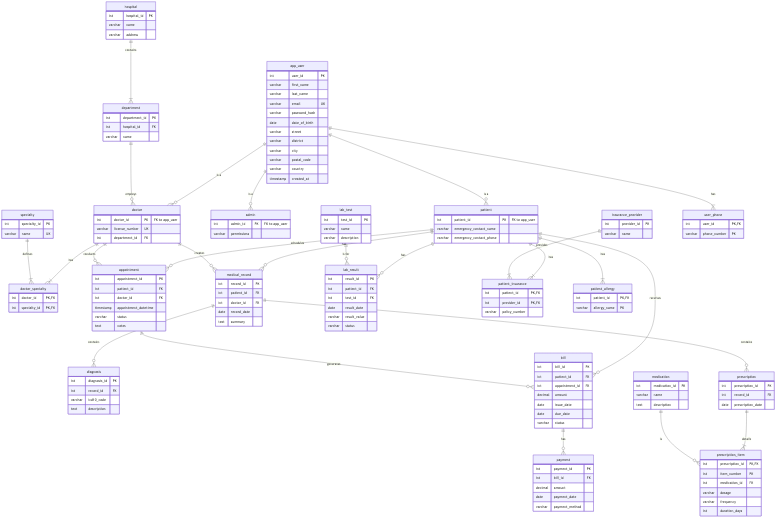
\includegraphics[width=\textwidth]{../er_diagram.png}
    \caption{Entity-Relationship (ER) Diagram.}
    \label{fig:er_diagram}
\end{figure}

\textit{Note: You need to export your Mermaid 'er\_diagram.mmd' as a PNG file and place it in the parent project folder.}

\subsection{Enhanced ER (EER) Diagram}
The Enhanced ER (EER) diagram extends the ER model with concepts like specialization and generalization. In our model, an \texttt{app\_user} supertype is specialized into \texttt{patient}, \texttt{doctor}, and \texttt{admin} subtypes.

\begin{figure}[h!]
    \centering
    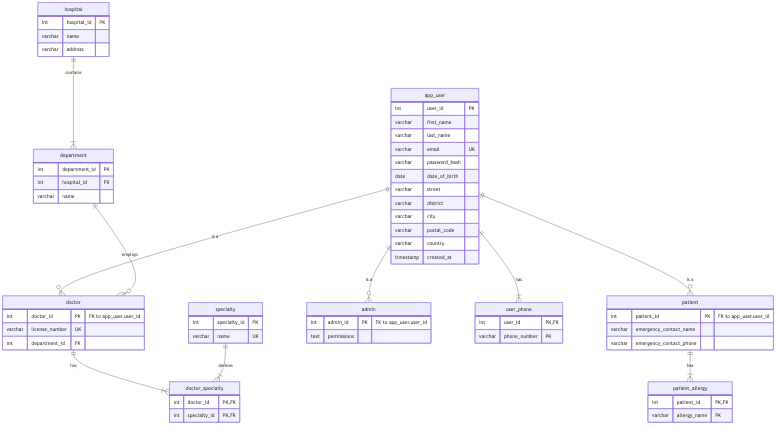
\includegraphics[width=\textwidth]{../eer_diagram.png}
    \caption{Enhanced Entity-Relationship (EER) Diagram.}
    \label{fig:eer_diagram}
\end{figure}

\textit{Note: You need to export your Mermaid 'eer\_diagram.mmd' as a PNG file and place it in the parent project folder.}

\subsubsection{Explanation of EER Concepts}
Here, we used specialization to model different types of users. For example, \texttt{doctor} and \texttt{patient} are specializations of a more general \texttt{app\_user} entity, inheriting common attributes like name and contact information while also having their own specific attributes.
